% Options for packages loaded elsewhere
\PassOptionsToPackage{unicode}{hyperref}
\PassOptionsToPackage{hyphens}{url}
%
\documentclass[
]{article}
\usepackage{amsmath,amssymb}
\usepackage{lmodern}
\usepackage{iftex}
\ifPDFTeX
  \usepackage[T1]{fontenc}
  \usepackage[utf8]{inputenc}
  \usepackage{textcomp} % provide euro and other symbols
\else % if luatex or xetex
  \usepackage{unicode-math}
  \defaultfontfeatures{Scale=MatchLowercase}
  \defaultfontfeatures[\rmfamily]{Ligatures=TeX,Scale=1}
\fi
% Use upquote if available, for straight quotes in verbatim environments
\IfFileExists{upquote.sty}{\usepackage{upquote}}{}
\IfFileExists{microtype.sty}{% use microtype if available
  \usepackage[]{microtype}
  \UseMicrotypeSet[protrusion]{basicmath} % disable protrusion for tt fonts
}{}
\makeatletter
\@ifundefined{KOMAClassName}{% if non-KOMA class
  \IfFileExists{parskip.sty}{%
    \usepackage{parskip}
  }{% else
    \setlength{\parindent}{0pt}
    \setlength{\parskip}{6pt plus 2pt minus 1pt}}
}{% if KOMA class
  \KOMAoptions{parskip=half}}
\makeatother
\usepackage{xcolor}
\usepackage[margin=1in]{geometry}
\usepackage{listings}
\newcommand{\passthrough}[1]{#1}
\lstset{defaultdialect=[5.3]Lua}
\lstset{defaultdialect=[x86masm]Assembler}
\usepackage{longtable,booktabs,array}
\usepackage{calc} % for calculating minipage widths
% Correct order of tables after \paragraph or \subparagraph
\usepackage{etoolbox}
\makeatletter
\patchcmd\longtable{\par}{\if@noskipsec\mbox{}\fi\par}{}{}
\makeatother
% Allow footnotes in longtable head/foot
\IfFileExists{footnotehyper.sty}{\usepackage{footnotehyper}}{\usepackage{footnote}}
\makesavenoteenv{longtable}
\usepackage{graphicx}
\makeatletter
\def\maxwidth{\ifdim\Gin@nat@width>\linewidth\linewidth\else\Gin@nat@width\fi}
\def\maxheight{\ifdim\Gin@nat@height>\textheight\textheight\else\Gin@nat@height\fi}
\makeatother
% Scale images if necessary, so that they will not overflow the page
% margins by default, and it is still possible to overwrite the defaults
% using explicit options in \includegraphics[width, height, ...]{}
\setkeys{Gin}{width=\maxwidth,height=\maxheight,keepaspectratio}
% Set default figure placement to htbp
\makeatletter
\def\fps@figure{htbp}
\makeatother
\setlength{\emergencystretch}{3em} % prevent overfull lines
\providecommand{\tightlist}{%
  \setlength{\itemsep}{0pt}\setlength{\parskip}{0pt}}
\setcounter{secnumdepth}{-\maxdimen} % remove section numbering
\ifLuaTeX
\usepackage[bidi=basic]{babel}
\else
\usepackage[bidi=default]{babel}
\fi
\babelprovide[main,import]{spanish}
% get rid of language-specific shorthands (see #6817):
\let\LanguageShortHands\languageshorthands
\def\languageshorthands#1{}
\usepackage{listings}
\usepackage{xcolor}

\definecolor{codegreen}{rgb}{0,0.6,0}
\definecolor{codeblue}{rgb}{0,0,0.6}
\definecolor{codegray}{rgb}{0.5,0.5,0.5}
\definecolor{codepurple}{rgb}{0.58,0,0.82}
\definecolor{backcolour}{rgb}{0.95,0.95,0.92}

\lstdefinestyle{mystyle}{
backgroundcolor=\color{backcolour},   
commentstyle=\color{codegreen},
keywordstyle=\color{magenta},
numberstyle=color{codeblue},
stringstyle=\color{codepurple},
breakatwhitespace=false,         
breaklines=true,                 
captionpos=b,                    
keepspaces=true,                 
showspaces=false,                
showstringspaces=false,
showtabs=false,                  
tabsize=2
}

\lstset{style = mystyle}

\ifLuaTeX
  \usepackage{selnolig}  % disable illegal ligatures
\fi
\IfFileExists{bookmark.sty}{\usepackage{bookmark}}{\usepackage{hyperref}}
\IfFileExists{xurl.sty}{\usepackage{xurl}}{} % add URL line breaks if available
\urlstyle{same} % disable monospaced font for URLs
\hypersetup{
  pdftitle={Predicción de la estructura secundaria de proteínas globulares},
  pdfauthor={Maria Lucas},
  pdflang={Es-es},
  hidelinks,
  pdfcreator={LaTeX via pandoc}}

\title{Predicción de la estructura secundaria de proteínas globulares}
\author{Maria Lucas}
\date{2023-03-24}

\begin{document}
\maketitle

{
\setcounter{tocdepth}{4}
\tableofcontents
}
\newpage

\hypertarget{algoritmo-k-nn}{%
\section{1. Algoritmo k-NN}\label{algoritmo-k-nn}}

El algoritmo k-nn (k-nearest neighbors) es un algoritmo de aprendizaje
supervisado utilizado para clasificación y regresión. En el proceso de
clasificación, el algoritmo busca encontrar la clase más común entre los
k ejemplos de entrenamiento más cercanos al punto de consulta. En el
proceso de regresión, el algoritmo busca encontrar el valor medio de los
k ejemplos de entrenamiento más cercanos al punto de consulta.

El funcionamiento del algoritmo k-nn es bastante sencillo. Primero, se
carga un conjunto de datos de entrenamiento que consta de entradas y
etiquetas correspondientes. Luego, se toma un punto de consulta (una
entrada sin etiquetar) y se calcula la distancia entre ese punto y cada
punto en el conjunto de datos de entrenamiento. Las distancias más
comunes utilizadas en k-nn son la distancia euclidiana y la distancia
Manhattan.

Una vez que se han calculado las distancias, se seleccionan los k puntos
de entrenamiento más cercanos al punto de consulta. Si se está
realizando clasificación, se seleccionan las etiquetas correspondientes
a estos puntos de entrenamiento y se toma la etiqueta más común como la
etiqueta asignada al punto de consulta. Si se está realizando regresión,
se toma el valor medio de las etiquetas de los k puntos de entrenamiento
más cercanos como el valor asignado al punto de consulta.

La elección del valor de k en el algoritmo k-nn es un factor crítico que
puede afectar significativamente el rendimiento del modelo. Si k es
demasiado pequeño, el modelo puede ser sensible al ruido en los datos y
puede sobreajustarse. Si k es demasiado grande, el modelo puede
subajustarse y no ser capaz de capturar patrones sutiles en los datos.
El valor de k dependerá del conjunto de datos y el problema específico
que se está abordando, aunque se puede empezar por la raíz cuadrada del
número de datos e ir ajustando.

\begin{longtable}[]{@{}
  >{\raggedright\arraybackslash}p{(\columnwidth - 2\tabcolsep) * \real{0.4167}}
  >{\raggedright\arraybackslash}p{(\columnwidth - 2\tabcolsep) * \real{0.5833}}@{}}
\toprule()
\begin{minipage}[b]{\linewidth}\raggedright
Ventajas
\end{minipage} & \begin{minipage}[b]{\linewidth}\raggedright
Inconvenientes
\end{minipage} \\
\midrule()
\endhead
Simple y fácil de interpretar & No produce un modelo \\
Rápida fase de entrenamiento & Lenta fase de clasificación \\
No paramétrico & Se debe escoger una k apropiada \\
Buen rendimiento en datos con pocos atributos & Computacionalmente
costoso para gran cantidad de datos \\
Se puede actualizar a tiempo real con nuevos datos & Sensible a datos
redundantes y a valores atípicos \\
& Requiere pre-procesamiento de los datos \\
\bottomrule()
\end{longtable}

\hypertarget{codificaciuxf3n-one-hot}{%
\section{2. Codificación one-hot}\label{codificaciuxf3n-one-hot}}

\begin{lstlisting}[language=Python]

def encode_sequence(sequence):
    
    # Define a dictionary that maps amino acids to their corresponding positions in the one-hot encoding
    aa_to_index = {'A': 0, 'R': 1, 'N': 2, 'D': 3, 'C': 4, 'Q': 5, 'E': 6, 'G': 7, 'H': 8, 'I': 9, 'L': 10, 'K': 11, 'M': 12, 'F': 13, 'P': 14, 'S': 15, 'T': 16, 'W': 17, 'Y': 18, 'V': 19}

    # Empty list to store the encoding
    encoding = [] 

    # Iterate over each amino acid in the sequence and encode it using the aa_to_index dictionary
    
    for aa in sequence:
        index = aa_to_index[aa]
        # Creates a list of 20 0 except for the element at the position of the index where it puts a 1
        # The extend method makes the new encoded aa be added to the encoding list
        encoding.extend([1 if i == index else 0 for i in range(20)])

    return encoding
\end{lstlisting}

\hypertarget{clasificador-knn}{%
\section{3. Clasificador knn}\label{clasificador-knn}}

\hypertarget{a-carga-del-fichero-y-tabla-resumen}{%
\subsection{(a) Carga del fichero y tabla
resumen}\label{a-carga-del-fichero-y-tabla-resumen}}

\begin{lstlisting}[language=Python]

# Loading data
import pandas as pd
data = pd.read_csv('data4.csv', delimiter=";").values
\end{lstlisting}

\begin{lstlisting}[language=Python]

# Summary table

def sum_table(data):
  
  # Defines 3 counters, one for each structure and initially sets them to 0
  coil = 0
  bsheet = 0
  ahelix = 0

  # Iterates over the sequence and adds 1 to the counter of the structure encountered
  for seq in data:
    # We use column -1 because it is where the structure info is located
    if seq[-1] == "_":
      coil += 1
    if seq[-1] == "e":
      bsheet += 1
    if seq[-1] == "h":
      ahelix += 1

  # Formats the table itself
  tabla = [["a-helix", ahelix], ["b-sheet", bsheet], ["coil", coil]]
  
  return print(tabulate(tabla, headers=["Estructura", "Contador"]))

# Apply the function

from tabulate import tabulate

sum_table(data)
\end{lstlisting}

\begin{lstlisting}
## Estructura      Contador
## ------------  ----------
## a-helix             2508
## b-sheet             1935
## coil                5557
\end{lstlisting}

\hypertarget{b-aplicaciuxf3n-one-hot}{%
\subsection{(b) Aplicación one-hot}\label{b-aplicaciuxf3n-one-hot}}

\begin{lstlisting}[language=Python]

import numpy as np

# Save the last column as y because they contain the structures to predict

y = data[:, -1]

# Removed the structures columns of the data
list_seq = np.delete(data, -1, 1)

# Create the list to store the encoded data
seq_encoded = []

# We iterate over the data applying the encoding function and storing it in the list
for seq in list_seq:
  seq_encoded.append(encode_sequence(seq))
\end{lstlisting}

\hypertarget{c-separaciuxf3n-de-los-datos}{%
\subsection{(c) Separación de los
datos}\label{c-separaciuxf3n-de-los-datos}}

\begin{lstlisting}[language=Python]

from sklearn.model_selection import train_test_split

# Transform the encoded list sequence to an array
seq_encoded = (np.array(seq_encoded))

# Split the data into training and testing sets setting the seed to 123
seq_encoded_train, seq_encoded_test, y_train, y_test = train_test_split(seq_encoded, y ,test_size=0.33,  random_state=123)

# Apply the sum function to examine the data sets
sum_table(y_test)
\end{lstlisting}

\begin{lstlisting}
## Estructura      Contador
## ------------  ----------
## a-helix              779
## b-sheet              692
## coil                1829
\end{lstlisting}

\begin{lstlisting}[language=Python]
sum_table(y_train)
\end{lstlisting}

\begin{lstlisting}
## Estructura      Contador
## ------------  ----------
## a-helix             1729
## b-sheet             1243
## coil                3728
\end{lstlisting}

\hypertarget{d-aplicaciuxf3n-k-nn-para-predecir-la-estructura}{%
\subsection{(d) Aplicación k-NN para predecir la
estructura}\label{d-aplicaciuxf3n-k-nn-para-predecir-la-estructura}}

\begin{lstlisting}[language=Python]
# Transform the training encoded list sequence to an array
seq_encoded_train = np.array(seq_encoded_train)

from sklearn.metrics import confusion_matrix, cohen_kappa_score, classification_report
from sklearn.neighbors import KNeighborsClassifier

# Create the list of k to study
k_list = [1, 3, 5, 7, 11]
# Defining list to store data
results = []
reports = []

# We iterate over the k list to generate a model for each k
for i in k_list:

  knn_i = KNeighborsClassifier(n_neighbors = i) # Creates the KNeighborsClassifier object with k=i
  knn_i.fit(seq_encoded_train, y_train) # Fit the model to the training set
  y_pred = knn_i.predict(seq_encoded_test) # Predicts the labels of the test data
  
  # We calculate the parameters to determine de adjust of the model:
  # Accuracy
  accuracy_i = knn_i.score(seq_encoded_test, y_test)
  
  # Kappa value
  kappa_i = cohen_kappa_score(y_test, y_pred)
  
  # Confusion matrix and order of the labels
  cm_i = confusion_matrix(y_test, y_pred, labels=["_", "e", "h"])
  order_i = knn_i.classes_
  
  # Error
  error_i = 1 - knn_i.score(seq_encoded_test, y_test)
  
  # Report
  report_i = classification_report(y_test, y_pred, labels=["_", "e", "h"])
  
  # Adds the parameters to the corresponding lists
  results.append([i, accuracy_i, kappa_i, error_i, cm_i, order_i])
  reports.append([i, report_i])
  
# Creates the results tables (out of the loop)
\end{lstlisting}

\begin{lstlisting}
## KNeighborsClassifier(n_neighbors=1)
## KNeighborsClassifier(n_neighbors=3)
## KNeighborsClassifier()
## KNeighborsClassifier(n_neighbors=7)
## KNeighborsClassifier(n_neighbors=11)
\end{lstlisting}

\begin{lstlisting}[language=Python]
tabla = tabulate(results, headers=["k", "Accuracy", "Kappa Value", "Error ", "Confusion matrix", "Class order"])
tabla2 = tabulate(reports, numalign = "right", stralign = "right", headers = ["k", "Others"])
# Prints the tables
print(tabla)
\end{lstlisting}

\begin{lstlisting}
##   k    Accuracy    Kappa Value    Error   Confusion matrix    Class order
## ---  ----------  -------------  --------  ------------------  -------------
##   1    0.759394       0.594782  0.240606  [[1497  162  170]   ['_' 'e' 'h']
##                                            [ 160  461   71]
##                                            [ 165   66  548]]
##   3    0.711212       0.491203  0.288788  [[1536  139  154]   ['_' 'e' 'h']
##                                            [ 271  359   62]
##                                            [ 275   52  452]]
##   5    0.682424       0.428372  0.317576  [[1551  143  135]   ['_' 'e' 'h']
##                                            [ 334  301   57]
##                                            [ 318   61  400]]
##   7    0.653636       0.366468  0.346364  [[1556  136  137]   ['_' 'e' 'h']
##                                            [ 362  266   64]
##                                            [ 374   70  335]]
##  11    0.625758       0.293059  0.374242  [[1593  109  127]   ['_' 'e' 'h']
##                                            [ 410  218   64]
##                                            [ 462   63  254]]
\end{lstlisting}

\begin{lstlisting}[language=Python]
print(tabla2)
\end{lstlisting}

\begin{lstlisting}
##   k                                                 Others
## ---  -----------------------------------------------------
##   1                precision    recall  f1-score   support
## 
##                 _       0.82      0.82      0.82      1829
##                 e       0.67      0.67      0.67       692
##                 h       0.69      0.70      0.70       779
## 
##          accuracy                           0.76      3300
##         macro avg       0.73      0.73      0.73      3300
##      weighted avg       0.76      0.76      0.76      3300
##   3                precision    recall  f1-score   support
## 
##                 _       0.74      0.84      0.79      1829
##                 e       0.65      0.52      0.58       692
##                 h       0.68      0.58      0.62       779
## 
##          accuracy                           0.71      3300
##         macro avg       0.69      0.65      0.66      3300
##      weighted avg       0.71      0.71      0.70      3300
##   5                precision    recall  f1-score   support
## 
##                 _       0.70      0.85      0.77      1829
##                 e       0.60      0.43      0.50       692
##                 h       0.68      0.51      0.58       779
## 
##          accuracy                           0.68      3300
##         macro avg       0.66      0.60      0.62      3300
##      weighted avg       0.67      0.68      0.67      3300
##   7                precision    recall  f1-score   support
## 
##                 _       0.68      0.85      0.76      1829
##                 e       0.56      0.38      0.46       692
##                 h       0.62      0.43      0.51       779
## 
##          accuracy                           0.65      3300
##         macro avg       0.62      0.56      0.57      3300
##      weighted avg       0.64      0.65      0.63      3300
##  11                precision    recall  f1-score   support
## 
##                 _       0.65      0.87      0.74      1829
##                 e       0.56      0.32      0.40       692
##                 h       0.57      0.33      0.42       779
## 
##          accuracy                           0.63      3300
##         macro avg       0.59      0.50      0.52      3300
##      weighted avg       0.61      0.63      0.59      3300
\end{lstlisting}

\hypertarget{e-predicciuxf3n-coilnon-coil-y-curva-roc}{%
\subsection{(e) Predicción coil/non-coil y curva
ROC}\label{e-predicciuxf3n-coilnon-coil-y-curva-roc}}

\begin{lstlisting}[language=Python]

# Define a function to summarise the data sets
def count_instances(array):
  # Counts unique ocurrences in the array
  unique, counts = np.unique(array, return_counts=True)
  # Shows them in a dictionary
  dic = dict(zip(unique, counts))
  
  return print(dic)
\end{lstlisting}

\begin{lstlisting}[language=Python]

# Preparing y
y2 = np.copy(y) # Copy y to y2 to preserve the original

# Change the structures (h and e to = 1, _ = 0), so 1 = nc, 0 = coil
y2[y2 == "h"] = "1"
y2[y2 == "e"] = "1"
y2[y2 == "_"] = "0"

# Examine the data set
count_instances(y2)

# Split the data set into training and test using the seed 123
\end{lstlisting}

\begin{lstlisting}
## {'0': 5557, '1': 4443}
\end{lstlisting}

\begin{lstlisting}[language=Python]
seq_encoded_train2, seq_encoded_test2, y2_train, y2_test = train_test_split(seq_encoded, y2 ,test_size=0.33,  random_state=123)

# Examine the data set
count_instances(y2_train)
\end{lstlisting}

\begin{lstlisting}
## {'0': 3728, '1': 2972}
\end{lstlisting}

\begin{lstlisting}[language=Python]
count_instances(y2_test)

#k-NN and ROC curve
\end{lstlisting}

\begin{lstlisting}
## {'0': 1829, '1': 1471}
\end{lstlisting}

\begin{lstlisting}[language=Python]
from sklearn.metrics import roc_curve, roc_auc_score

# Create the list of k to study
k_list = [1, 3, 5, 7, 11]

# Defining list to store data
results_list2 = []
roc_auc_list = []
fpr_list = []  # False positive ratio
tpr_list = []  # True positive Ratio

# We iterate over the k list to generate a model for each k
for i in k_list:
  
  knn_i = KNeighborsClassifier(n_neighbors=i) # Creates the KNeighborsClassifier object with k=i
  knn_i.fit(seq_encoded_train2, y2_train) # Fit the model to the training set
  y_pred_proba = knn_i.predict_proba(seq_encoded_test2)[:, 1]  # Predicted probabilities of class 1
  y_pred = np.where(y_pred_proba >= 0.5, '1', '0')  # Convert predicted probabilities to binary class labels
  
  # Calculate the parameters to create roc_curve
  fpr, tpr, thresholds = roc_curve(y2_test, y_pred_proba, pos_label = "1")
  # Calculate ROC_curve
  roc_auc = roc_auc_score(y2_test, y_pred_proba)
  
  # We calculate the parameters to determine de adjust of the model:
  # Accuracy
  accuracy_i = knn_i.score(seq_encoded_test2, y2_test)
  
  #Kappa Value
  kappa_i = cohen_kappa_score(y2_test, y_pred)
  
  # Confusion matrix and order of the labels
  cm_i = confusion_matrix(y2_test, y_pred, labels=["0", "1"])
  order_i = knn_i.classes_
  
  # Error
  error_i = 1 - accuracy_i
  
  # Adds the parameters to the results list
  results_list2.append([i, accuracy_i, kappa_i, error_i, cm_i ,order_i])
  
  # Adds the ROC curve, fpr and tpr to the list
  roc_auc_list.append(roc_auc)
  fpr_list.append(fpr)  # add fpr for this value of k to the list
  tpr_list.append(tpr)  # add tpr for this value of k to the list

# Creates the table to show the parameters
\end{lstlisting}

\begin{lstlisting}
## KNeighborsClassifier(n_neighbors=1)
## KNeighborsClassifier(n_neighbors=3)
## KNeighborsClassifier()
## KNeighborsClassifier(n_neighbors=7)
## KNeighborsClassifier(n_neighbors=11)
\end{lstlisting}

\begin{lstlisting}[language=Python]
tabla = tabulate(results_list2, headers=["k", "Accuracy", "Kappa Value", "Error ", "Confusion matrix", "Class order"])
print(tabla) # Prints the table

# Plots the ROC curves
\end{lstlisting}

\begin{lstlisting}
##   k    Accuracy    Kappa Value    Error   Confusion matrix    Class order
## ---  ----------  -------------  --------  ------------------  -------------
##   1    0.800909       0.597264  0.199091  [[1497  332]        ['0' '1']
##                                            [ 325 1146]]
##   3    0.754545       0.502118  0.245455  [[1441  388]        ['0' '1']
##                                            [ 422 1049]]
##   5    0.730909       0.451173  0.269091  [[1443  386]        ['0' '1']
##                                            [ 502  969]]
##   7    0.709697       0.407354  0.290303  [[1415  414]        ['0' '1']
##                                            [ 544  927]]
##  11    0.680909       0.346082  0.319091  [[1396  433]        ['0' '1']
##                                            [ 620  851]]
\end{lstlisting}

\begin{lstlisting}[language=Python]
import matplotlib.pyplot as plt

plt.figure(figsize=(8, 6)) # Set figure size
for i in range(len(k_list)): # Draw as many curves as items in k_list
    plt.plot(fpr_list[i], tpr_list[i], label='k = %d, AUC = %.2f' % (k_list[i], roc_auc_list[i])) # Plots the curve for each k and sets the AUC values for the legend
plt.plot([0, 1], [0, 1], 'k--') # Draws axis
plt.xlim([0.0, 1.0]) # Set X axis
\end{lstlisting}

\begin{lstlisting}
## (0.0, 1.0)
\end{lstlisting}

\begin{lstlisting}[language=Python]
plt.ylim([0.0, 1.05]) # Set Y axis
\end{lstlisting}

\begin{lstlisting}
## (0.0, 1.05)
\end{lstlisting}

\begin{lstlisting}[language=Python]
plt.xlabel('False Positive Rate (1-E)') # X label
plt.ylabel('True Positive Rate (S)') # Y label
plt.title('ROC Curve for k-NN Classifier') # Graph title
plt.legend(loc="lower right") # Legend
plt.show() # Prints the graph
\end{lstlisting}

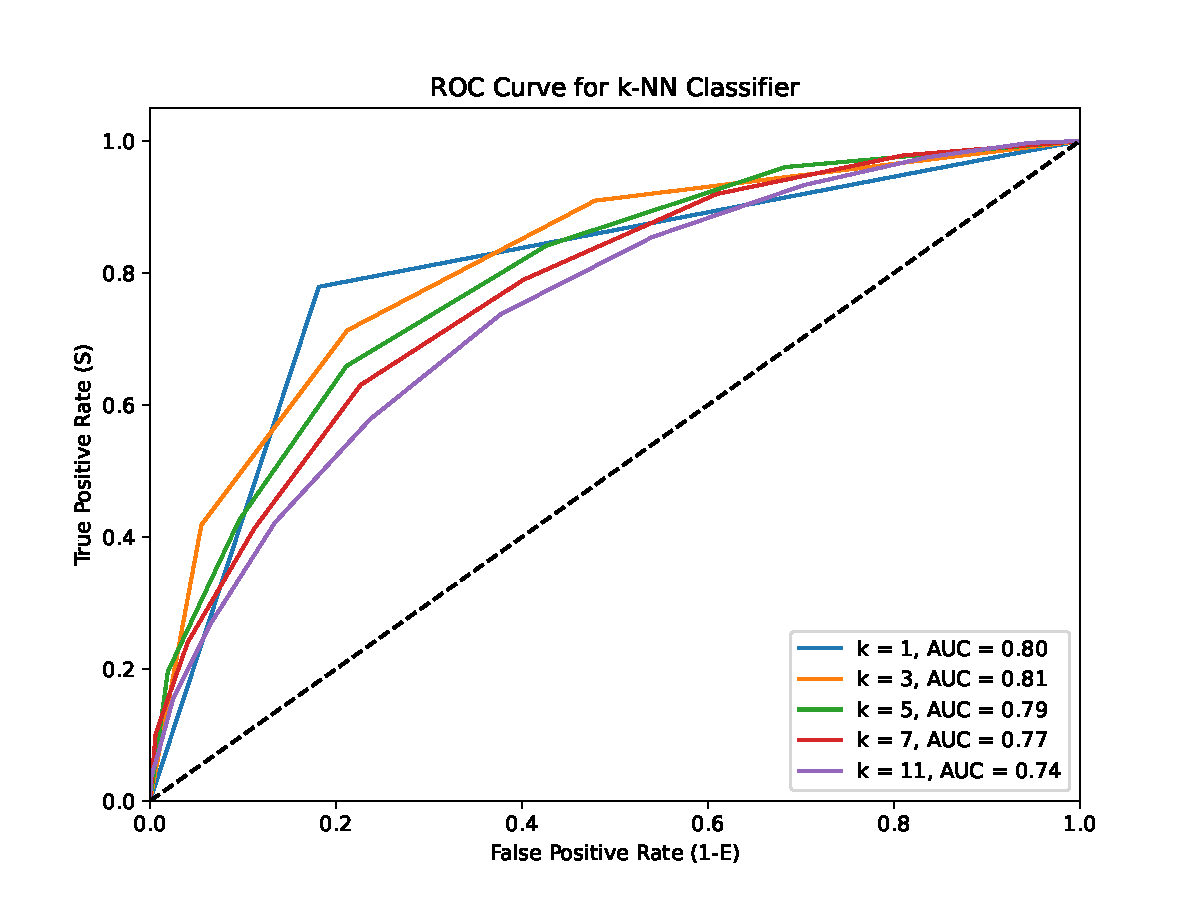
\includegraphics{code_files/figure-latex/unnamed-chunk-9-1.pdf}

\hypertarget{f-resultados}{%
\subsection{(f) Resultados}\label{f-resultados}}

\hypertarget{clasificaciuxf3n-para-tres-estructuras}{%
\subsubsection{Clasificación para tres
estructuras}\label{clasificaciuxf3n-para-tres-estructuras}}

Previamente a la aplicación del algoritmo, es conveniente asegurarse que
todos los tipos de estructura están correctamente representados tanto en
el set de entrenamiento como en el de test, ya que por azar podrían
haberse repartido todos los de una clase en el set de test y nuestro
modelo nunca los precedería. Como podemos observar no tenemos ese
problema ya se repartieron de forma bastante equitativa. También cabe
destacar le clase coil está más representada con respecto al resto.

Observando los resultados de la clasificación para las tres clases de
estructuras secundarias, podemos ver que el modelo que mejor predice es
el que usa k=1. Podemos deducirlo puesto que tiene un error de
clasificación menor (0,24) lo que indica que tan solo predice mal un
24\% de los casos del data test. Como bien sabemos este error no deja de
ser 1-exactitud (accuracy), así que estos dos parámetros nos aportan la
idea de qué tan bien nuestro modelo clasifica la estructura de la cadena
de aminoácidos.

El valor kappa está estrechamente relacionado con la exactitud, excepto
que éste tiene en cuenta la probabilidad de clasificar correctamente por
azar. Cuánto más cercano a 1 es el valor, mejor predice el modelo,
mientras que si el valor es cercano a 0, el modelo no predice mejor que
una clasificación aleatoria. En este caso el valor más elevado es el de
k=1, con 0.59. Si seguimos la guía general proporcionada en el libro, el
modelo sigue un ajuste moderado-bueno. Depende de la aplicación del
modelo si este ajuste es suficientemente bueno para ser usado o no,
según si se pueden permitir errores o no.

La precisión, el recall y el F-score también parecen indicar que el
modelo con k=1 se ajusta mejor. En este caso como hay 3 posibles
resultados se calculan sobre cada una de las clases. Aunque el k=1
parezca ajustarse mejor, escogemos el modelo según la naturaleza de
nuestros datos y el problema a resolver. La precisión representa la
proporción de ejemplos positivos que eran realmente positivos (que se
han clasificado como esa clase y lo eran). Si queremos que el modelo
sólo clasifique coil en los casos que realmente sea coil, buscaremos un
valor alto de precisión para coil. Por otro lado, un valor elevado de
recall indicará que nuestro modelo detecta gran parte de los casos
positivos, siguiendo el ejemplo anterior, de todas las estructuras que
eran coil ha clasificado bien muchas de ellas. Finalmente, si queremos
hacernos una idea general podemos consultar el F-score, que combina
recall y precisión en un solo valor.

Cabe destacar que ninguno de los parámetros que hemos mencionado por sí
solos puede proporcionar una idea clara de si un modelo está overfitted
o underfitted a los datos, ya que cada uno de ellos mide diferentes
aspectos del rendimiento del modelo. En general, se recomienda evaluar
varios parámetros diferentes y realizar una evaluación cruzada para
evitar overfitting.

\hypertarget{clasificaciuxf3n-para-coil-y-non-coil}{%
\subsubsection{Clasificación para coil y
non-coil}\label{clasificaciuxf3n-para-coil-y-non-coil}}

Primeramente, cabe destacar que al separar los datos de esta manera, la
clase non-coil está mejor representada que las clases a-helix y b-sheet
por separado, así que a priori, pensaríamos que obtendremos un mejor
modelo.

Igual que en el modelo anterior, parece ser que el k=1 es el más exacto
y con menor error. Nuevamente el valor kappa nos indica que estamos ante
un modelo de ajuste moderado-bueno. En este caso no examinamos los
valores de precisión y recall, ya que al tener sólo dos posibles
resultados equivalen a Valor Predictivo Positivo y Sensibilidad, que
examinaremos más cómodamente mediante curvas ROC.

Analizando la curva ROC podría parecer que k=1 es el que mejor se
ajusta, ya que es el que más se aproxima a 1 de sensibilidad y 0 de 1 -
especificidad. El modelo parece clasificar de forma bastante equilibrada
los verdaderos positivos sin elevar mucho el número de falsos positivos.
Lo mismo sucede con los negativos. Lo podemos ver en la propia curva
ROC, pero también en la propia matriz de confusión. El número de falsos
positivos y de falsos negativos es bastante similar, sobretodo para k=1.

Pero si examinamos el AUC, vemos que k = 3 es ligeramente superior. Al
ser una diferencia de tan solo 0.01, al tener en cuenta el resto de
factores, k=1 es el modelo que mejor se ajusta. Consultando el libro de
referencia, podemos determinar que el ajuste es bueno/excelente.

\hypertarget{comentario-global}{%
\subsubsection{Comentario global}\label{comentario-global}}

En ambos casos hemos obtenido un relativamente buen modelo para predecir
la estructura de la secuencia de aminoácidos. Parecería que el modelo
coil/non-coil sería más exacto al sólo tener dos posibles resultados en
lugar de tres, pero tras examinar los distintos parámetros vemos que en
realidad ambos modelos son buenos.

Un valor de k muy pequeño como es k=1, puede significar que el modelo
está muy ajustado a los datos de entrenamiento (overfitted) y no
generalizará bien con datos nuevos. Si quisiéramos ajustar mejor los
modelos necesitaríamos usar técnicas como las cross-validation para usar
el máximo número de datos posibles para su entrenamiento. También sería
conveniente una vez tengamos el modelo que queremos utilizar, después de
ajustar la k y las estructuras a predecir, que creemos un set de datos
de validación para asegurarnos que efectivamente el modelo es bueno. Al
usar el mismo test en todos los modelos para estudiar su ajuste, hemos
escogido el test que mejor predice esos datos, que podría no ser el que
mejor prediga datos futuros. Pasando un nuevo set de datos de validación
(``nunca vistos'') nos dará idea de cómo de bien predice datos el modelo
final.

\end{document}
